%% LyX 2.3.6.1 created this file.  For more info, see http://www.lyx.org/.
%% Do not edit unless you really know what you are doing.
\documentclass[english]{article}
\usepackage[T1]{fontenc}
\usepackage[latin9]{inputenc}
\usepackage{url}
\usepackage{amsmath}
\usepackage{graphicx}

\makeatletter

%%%%%%%%%%%%%%%%%%%%%%%%%%%%%% LyX specific LaTeX commands.
%% Because html converters don't know tabularnewline
\providecommand{\tabularnewline}{\\}

%%%%%%%%%%%%%%%%%%%%%%%%%%%%%% Textclass specific LaTeX commands.
\newenvironment{lyxcode}
	{\par\begin{list}{}{
		\setlength{\rightmargin}{\leftmargin}
		\setlength{\listparindent}{0pt}% needed for AMS classes
		\raggedright
		\setlength{\itemsep}{0pt}
		\setlength{\parsep}{0pt}
		\normalfont\ttfamily}%
	 \item[]}
	{\end{list}}

\makeatother

\usepackage{babel}
\usepackage{listings}
\renewcommand{\lstlistingname}{Listing}

\begin{document}
\title{QFC: a parallel software tool for feature construction, based on Grammatical
Evolution}
\author{Ioannis G. Tsoulos}
\date{Department of Informatics and Telecommunications, University of Ioannina,
47100 Arta, Greece }
\maketitle
\begin{abstract}
This paper presents and analyzes a programming tool that implements
a method for classification and function regression problems. This
method builds new features from existing ones with the assistance
of a hybrid algorithm that makes use of artificial neural networks
and Grammatical Evolution. The implemented software exploits modern
multi-core computing units for faster execution. The method has been
applied to a variety of classification and function regression problems
and an extensive comparison with other methods of computational intelligence
is made.
\end{abstract}

\section{Introduction }

Many problems from various research areas can be considered as classification
or regression problems, such as problems from physics \cite{fc_physics1,nnphysics1,nnphysics2,nnphysics3},
chemistry \cite{fc_chem1,fc_chem2,fc_chem3}, economics \cite{fc_econ1,fc_econ2},
pollution \cite{fc_pollution1,fc_pollution2,fc_pollution3}, medicine
\cite{nnmed1,nnmed2} etc. These problems are usually tackled by learning
models such as Artificial Neural Networks \cite{nn1,nn2}, Radial
Basis Function (RBF) networks \cite{rbf1,rbf2}, Support Vector Machines
(SVM) \cite{svm}, etc. A review of the methods used in classification
can be found in the work of Kotsiantis et al \cite{class_review}. 

Learning data is usually divided into two parts: training data and
test data. Learning models adjust their parameters, taking the training
data as input and are evaluated on the test data. The number of learning
model parameters directly depends on the dimension of the input problem
(number of features) and this means that for large problems, large
amounts of memory are required to store and manage the learning models.
In addition, as the number of parameters of the computational models
grows, a longer time is required to adjust the parameters. Also, as
the dimension of the data grows, more samples (patterns) are required
in order to achieve high learning rates. A discussion on how the dimensionality
of the input problems affects the effectiveness of neural networks
is presented in  \cite{nndimension}. A common approach to reduce
the dimension of the input data is the Principal Component Analysis
(PCA) technique \cite{nnpca1,nnpca2,nnpca3} or the Minimum redundancy
feature selection (MRMR) technique \cite{mrmr1,mrmr2}. Also, Wang
et al \cite{nn_autoencoder} proposed an auto-encoder based dimensionality
reduction method for large datasets. An overview of dimensionality
reduction techniques can be found in the work of Ayesha et al \cite{reduction_comparison}.

The current article describes the method and the software associated
with a feature construction method based on Grammatical Evolution
\cite{ge_main}, which is an evolutionary process that can create
programs in any programming language. This process has been used in
a variety of cases, such as automatic composition of music \cite{ge_music},
construction of neural networks \cite{ge_nn,ge_nn2}, automatic constant
creation \cite{ge_constant}, evolution of video games \cite{ge_pacman},
energy demand estimation \cite{ge_energy} etc. The described method
constructs subsets of features from the original ones using non-linear
combinations of them. The method is graphically illustrated in Figure
\ref{fig:Schematic-representation-of}.\textbf{ }Initially, the method
was described in \cite{fc1} and it has been utilized in a variety
of cases, such as Spam Identification \cite{fc2},\textbf{ }Fetal
heart classification \cite{fc3}, epileptic oscillations in clinical
intracranial electroencephalograms \cite{fc4}, classification of
EEG signals \cite{fc5} etc.

The proposed software has been implemented in ANSI C++ utilizing the
freely available library of QT from \url{https://www.qt.io}. The
user should supply the training and test data of the underlying problem
as well as the desired number of features that will be created. The
evaluation of the constructed features can be made using a variety
of machine learning models and the user can easily extend the software
to add more learning models. Also, the software has a variety of command
line options to control the parameters of the learning models or to
manage the output of the method. Finally, since the process of Grammatical
Evolution can require a lot of execution time, parallel computation
is included in the proposed software through the OpenMP programming
library \cite{openmp}. 

The rest of this article is organized as follows: in section \ref{sec:Methods}
the proposed method is analyzed, in section \ref{sec:The-software}
the proposed software is outlined in detail, in section \ref{sec:Experiments}
a variety of experiments are conducted and presented and finally in
section \ref{sec:Conclusions} some conclusions and future guidelines
are discussed.

\begin{figure}
\caption{Schematic representation of the feature construction technique.\label{fig:Schematic-representation-of}}

\centering{}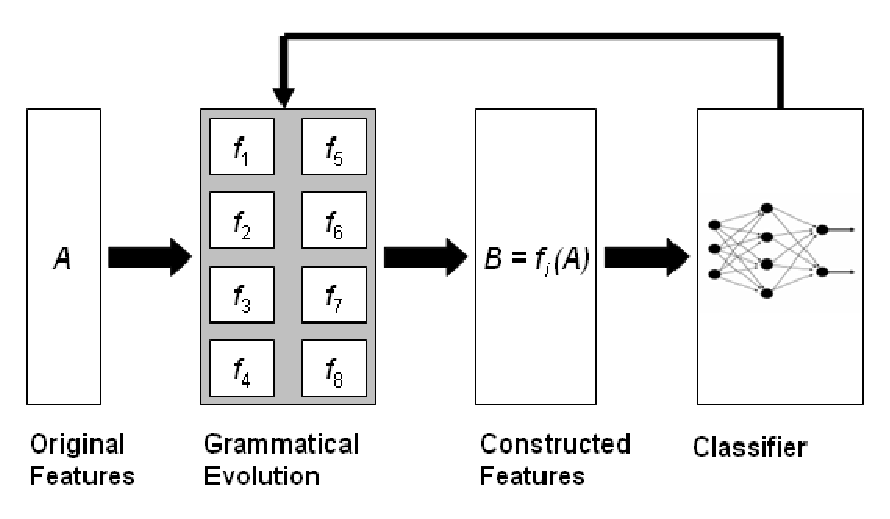
\includegraphics[scale=0.7]{fc_schema}
\end{figure}


\section{Methods \label{sec:Methods}}

The proposed technique is divided into two phases: in the first phase,
new features are constructed from the old ones using Grammatical Evolution
and in the second phase these new features modify the control set
and a machine learning model is applied to the new control set.

\subsection{Grammatical Evolution}

Grammatical evolution is a biologically inspired procedure that can
create artificial programs in any language. In Grammatical evolution
the chromosomes enclose production rules from a BNF (Backus--Naur
form) grammar\cite{bnf1}. These grammars usually described as a set
\textbf{$G=\left(N,T,S,P\right)$}, where
\begin{itemize}
\item \textbf{$N$ }is the set of non-terminal symbols.
\item \textbf{$T$ }is the set of terminal symbols.\textbf{ }
\item $S$ is a non-terminal symbol defined as the start symbol of the grammar.
\item \textbf{$P$ }is a set of production rules in the form \textbf{$A\rightarrow a$
}or\textbf{ $A\rightarrow aB,\ A,B\in N,\ a\in T$.}
\end{itemize}
In order for Grammatical Evolution to work, the original grammar is
expanded by enumerating all production rules. For example, consider
the modified grammar of Figure \ref{fig:BNF-grammar-of}. The symbols
that are in <> are considered as non-terminal symbols. The numbers
in parentheses are the production sequence numbers for each non-terminal
symbol. The constant N is the original number of features for the
input data. In Grammatical Evolution, the chromosomes are expressed
as vectors of integers. Every element of each chromosome denotes a\textbf{
}production rule from the provided BNF grammar. The algorithm starts
from the start symbol of the grammar and gradually produces some program
string, by replacing non - terminal symbols with the right hand of
the selected production rule. The selection of the rule has two steps:
\begin{itemize}
\item Take the next element from the chromosome and denote it as V.
\item Select the next production rule according to the the scheme Rule =
V mod R, where R is the number of production rules for the current
non -- terminal symbol. 
\end{itemize}
For example, consider the chromosome chromosome $x=\left[9,8,6,4,16,10,17,23,8,14\right]$
and $N=3$. The steps of mapping this chromosome to the valid expression\textbf{
$f(x)=x_{2}+\cos\left(x_{3}\right)$ }are illustrated in Table \ref{tab:table_with_steps}. 

\begin{figure}
\caption{BNF grammar of the proposed method.\label{fig:BNF-grammar-of}}

\begin{lyxcode}
S::=<expr>~~~(0)~

<expr>~::=~~(<expr>~<op>~<expr>)~~(0)~~~~~~~~~~~~~

~~~~~~~~~~~|~<func>~(~<expr>~)~~~~(1)~~~~~~~~~~~~~

~~~~~~~~~~~|<terminal>~~~~~~~~~~~~(2)~

<op>~::=~~~~~+~~~~~~(0)~~~~~~~~~~~~~

~~~~~~~~~~~|~-~~~~~~(1)~~~~~~~~~~~~~

~~~~~~~~~~~|~{*}~~~~~~(2)~~~~~~~~~~~~~

~~~~~~~~~~~|~/~~~~~~(3)

<func>~::=~~~sin~~(0)~~~~~~~~~~~~~

~~~~~~~~~~~|~cos~~(1)~~~~~~~~~~~~~

~~~~~~~~~~~|exp~~~(2)~~~~~~~~~~~~~

~~~~~~~~~~~|log~~~(3)

<terminal>::=<xlist>~~~~~~~~~~~~~~~~(0)~~~~~~~~~~~~~~~~~~~~~~

~~~~~~~~~~~|<digitlist>.<digitlist>~(1)

<xlist>::=x1~~~~(0)~~~~~~~~~~~~~~

~~~~~~~~~~~|~x2~(1)~~~~~~~~~~~~~~

~~~~~~~~~~~\dots \dots \dots{}~~~~~~~~~~~~~

~~~~~~~~~~~|~xN~(N)

<digitlist>::=<digit>~~~~~~~~~~~~~~~~~~(0)~~~~~~~~~~~~~~~~~

~~~~~~~~~~~|~<digit><digit>~~~~~~~~~~~~(1)

~~~~~~~~~~~|~<digit><digit><digit>~~~~~(2)

<digit>~~::=~0~(0)~~~~~~~~~~~~~

~~~~~~~~~~~|~1~(1)~~~~~~~~~~~~~

~~~~~~~~~~~|~2~(2)~~~~~~~~~~~~~

~~~~~~~~~~~|~3~(3)~~~~~~~~~~~~~

~~~~~~~~~~~|~4~(4)~~~~~~~~~~~~~

~~~~~~~~~~~|~5~(5)~~~~~~~~~~~~~

~~~~~~~~~~~|~6~(6)~~~~~~~~~~~~~

~~~~~~~~~~~|~7~(7)~~~~~~~~~~~~~

~~~~~~~~~~~|~8~(8)~~~~~~~~~~~~~

~~~~~~~~~~~|~9~(9)
\end{lyxcode}
\end{figure}
\begin{table}
\caption{Steps to produce a valid expression from the BNF grammar.\label{tab:table_with_steps}}

\begin{tabular}{|c|c|c|}
\hline 
String & Chromosome & Operation\tabularnewline
\hline 
\hline 
<expr> & 9,8,6,4,16,10,17,23,8,14 & $9\mod3=0$\tabularnewline
\hline 
(<expr><op><expr>) & 8,6,4,16,10,17,23,8,14 & $8\mod3=2$\tabularnewline
\hline 
(<terminal><op><expr>) & 6,4,16,10,17,23,8,14 & $6\mod2=0$\tabularnewline
\hline 
(<xlist><op><expr>) & 4,16,10,17,23,8,14 & $4\mod3=1$\tabularnewline
\hline 
(x2<op><expr>) & 16,10,17,23,8,14 & $16\mod4=0$\tabularnewline
\hline 
(x2+<expr>) & 10,17,23,8,14 & $10\mod3=1$\tabularnewline
\hline 
(x2+<func>(<expr>)) & 17,23,8,14 & $17\mod4=1$\tabularnewline
\hline 
(x2+cos(<expr>)) & 23,8,14 & $23\mod2=1$\tabularnewline
\hline 
(x2+cos(<terminal>)) & 8,14 & $8\mod2=0$\tabularnewline
\hline 
(x2+cos(<xlist>)) & 14 & $14\mod3=2$\tabularnewline
\hline 
(x2+cos(x3)) &  & \tabularnewline
\hline 
\end{tabular}
\end{table}


\subsection{The feature construction procedure\label{subsec:The-feature-construction}}

The following procedure is executed in order to produce $N_{f}$ features
from the original ones for a given chromosome $X$:
\begin{enumerate}
\item \textbf{Split} $X$ into $N_{f}$ parts.
\item \textbf{For} $i=1..N_{f}$ \textbf{denote} each part as $x_{i}$.
\item \textbf{For} every part $x_{i}$ construct a feature $\mbox{FT}_{i}$
using the grammar given in \ref{fig:BNF-grammar-of}
\end{enumerate}
Every feature $\mbox{FT}_{i}$ is considered as a mapping function,
that transforms the original features to a new one. For example the
feature 
\[
\mbox{FT}_{1}=x_{1}^{2}+\sin(\left(x_{2}\right)
\]
is a non - linear function that maps the original feature $\left(x_{1},x_{2}\right)$
into $\mbox{FT}_{1}$. Let $\left(x_{1},x_{2}\right)=\left(2,1\right)$.
The mapping procedure will create the value $4+\sin(1)$.

\subsection{The feature construction step }

The method has the following steps:
\begin{enumerate}
\item \textbf{Initialization} step. \textbf{}

\begin{enumerate}
\item \textbf{Read} the train data. The train data contains $M$ patterns
as pairs $\left(x_{i},t_{i}\right),\ i=1..M$ where $t_{i}$ is the
actual output for pattern $x_{i}$.
\item \textbf{Set $N_{G}$}, the maximum number of generations.
\item \textbf{Set $N_{C}$}, the number of chromosomes.
\item \textbf{Set $p_{S}$}, the selection rate.
\item \textbf{Set} $N_{f}$, the desired number of features. 
\item \textbf{Set $p_{M}$}, the mutation rate.
\item \textbf{Initialize} the chromosomes of the population. Every element
of each chromosome is initialized randomly in the range {[}0,255{]}.
\item \textbf{Set} iter=1
\end{enumerate}
\item \textbf{Genetic step}

\begin{enumerate}
\item \textbf{For $i=1,\ldots,N_{g}$ do}

\begin{enumerate}
\item \textbf{Create} using the procedure of subsection \ref{subsec:The-feature-construction}
a set of $N_{f}$ for the corresponding chromosome $g_{i}$. 
\item \textbf{Transform} the original train data to the new train data using
the previously created features. Denote the new train set as $\left(x_{g_{i},j},t_{j}\right),\ j=1,..M$
\item \textbf{Apply }a learning model $C$ (such as RBF) to the new data
and \textbf{calculate} the fitness $f_{i}$ as
\begin{equation}
f_{i}=\sum_{j=1}^{M}\left(C\left(x_{g_{i},j}\right)-t_{j}\right)^{2}
\end{equation}
\item \textbf{Apply} the selection procedure. During selection, the chromosomes
are classified according to their fitness. The best\textbf{ $\left(1-p_{s}\right)\times N_{C}$}
chromosomes are transferred without changes to the next generation
of the population. The rest will be replaced by chromosomes that will
be produced at the crossover.
\item \textbf{Apply} the crossover procedure.\textbf{ }During this process,
$p_{s}\times N_{c}$ chromosomes will be created. Firstly, for every
pair of produced offsprings, two distinct chromosomes (parents) are
selected from the current population using tournament selection: First,
a subset of $K>1$ randomly selected chromosomes is created and the
chromosome with the best fitness value is selected as parent.\textbf{
}For every pair $(z,w)$ of parents, two new offsprings $\tilde{z}$
and $\tilde{w}$ are created through one point crossover as graphically
shown in Figure \ref{fig:onepoint}.
\item \textbf{Apply} the mutation procedure. For every element of each chromosome,
select a random number $r\in\left[0,1\right]$ and alter the corresponding
chromosome if $r\le p_{m}$.
\end{enumerate}
\item \textbf{EndFor}
\end{enumerate}
\item \textbf{Set} iter=iter+1
\item \textbf{If} $\mbox{iter}\le N_{G}$ goto \textbf{Genetic} Step, else
\textbf{terminate} and obtain $g^{*}$ as the best chromosome in the
population.

\end{enumerate}
\begin{figure}
\caption{Example of one - point crossover.\label{fig:onepoint}}

\centering{}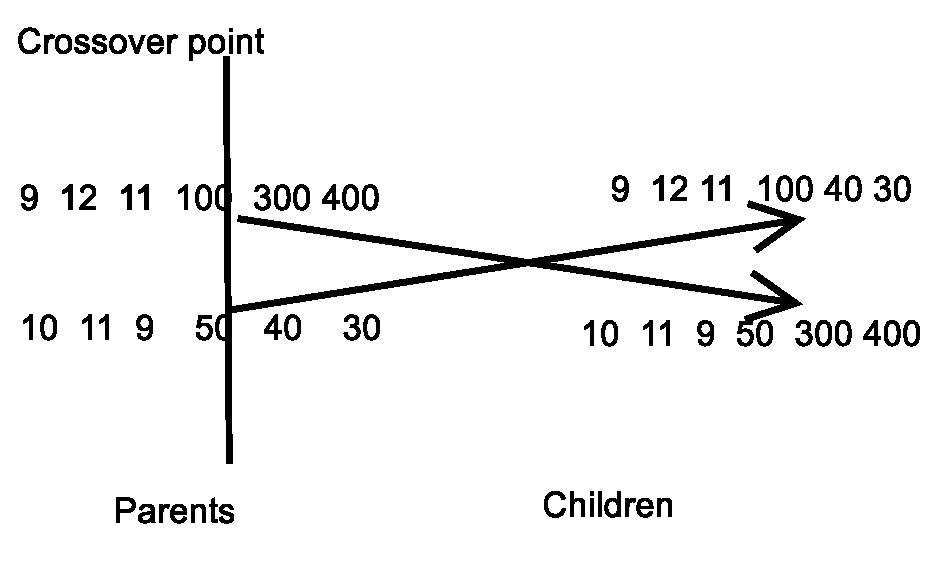
\includegraphics[scale=0.6]{cross}
\end{figure}


\subsection{The feature evaluation step}

During the feature evaluation step, the following steps are executed:
\begin{enumerate}
\item \textbf{Denote} as $T=\left(x_{i},y_{i}\right),\ i=1,..,K$ the original
test set. 
\item \textbf{Obtain} the best chromosome $g^{*}$ of the feature construction
step.
\item \textbf{Construct} $N_{f}$ features for $g^{*}$ using the procedure
of subsection \ref{subsec:The-feature-construction}.
\item \textbf{Transform} $T$ into $T'=\left(x_{g^{*},i},y_{i}\right),\ i=1,..,K$
using the previously constructed features.
\item \textbf{Apply} a learning model such as RBF or a neural network to
$T'$ and obtain the test error.
\end{enumerate}

\section{The software\label{sec:The-software}}

\subsection{Installation procedure }

The software is entirely written in ANSI C++ using the freely available
QT programming library. The library can be downloaded from \url{https://www.qt.io}
As expected, the software can be installed on the majority of operating
systems, even on mobile devices (Android, Ios etc). The program is
freely available from \url{https://github.com/itsoulos/QFc} and the
user should issue the following commands under most UNIX systems to
compile the project:
\begin{enumerate}
\item Download QFc-master.zip from the above url
\item gunzip QFc-master.zip
\item cd QFc
\item qmake .
\item make
\end{enumerate}
The final outcome of the previous steps is a command line program
called \emph{qfc}.

\subsection{Data format }

Classification and regression problems should be formatted in files
according to the format shown in Figure \ref{fig:Example-of-input}.\textbf{
}The integer number D denotes the number of features of the dataset
and M\textbf{ }represents the number of patterns. In every  subsequent
line of the file there should be the input pattern and the final column
is the real output (category) for the corresponding pattern. 

\begin{figure}
\caption{Example of input file for regression/classification.\label{fig:Example-of-input}}

D

M

$\begin{array}{ccccc}
x_{11} & x_{12} & \ldots & x_{1D} & y_{1}\\
x_{21} & x_{22} & \ldots & x_{2D} & y_{2}\\
\vdots & \vdots & \vdots & \vdots & \vdots\\
x_{M1} & x_{M2} & \ldots & x_{MD} & y_{M}
\end{array}$
\end{figure}


\subsection{The program qfc }

The program \emph{qfc} has a variety of command line options. All
options are in form $--$key=value, where key is the name of the option
and value is the actual option value. The main options of the program
are:
\begin{enumerate}
\item $--$trainFile=filename, where filename is the full path to data containing
the input train set. The file must be in the format of Figure \ref{fig:Example-of-input}.
\item $--$testFile=filename, where filename is the full path to data containing
the input test set. The format of this file should be the same as
the train data. The user should at least provide the train and test
set in order to execute the program.
\item $--$features=n, set as the n the number of features that will be
constructed by the method. The default value is 1.
\item $--$randomSeed=r, set as r the random seed generator. The default
value for this parameter is 1 and the drand48() random generator of
c++ language was used.
\item $--$featureCreateModel=model, the string parameter model sets the
name of the used feature construction model. The default value is
``rbf'' and accepted values are: 
\begin{enumerate}
\item \textbf{copy}. With this value, no feature construction is done and
the original data set is used for training by the model specified
by the option $--$featureEvaluateModel.
\item \textbf{rbf}. This value is used to utilize a Radial Basis Function
neural network for the evaluation of the constructed features.
\item \textbf{neural}. This value is used to use a neural network for the
evaluation of the constructed features. 
\item \textbf{knn}. A simple K-nearest neighbor (KNN) method is used \cite{knn}. 
\item \textbf{osamaRbf}. A simple RBF implementation as downloaded from
\url{https://github.com/osama-afifi/RBF-Radial-Basis-Function-Network}.
\end{enumerate}
\item $--$featureEvaluateModel=model, the string parameter model sets the
name of the used model for the evaluation of the constructed features.
The default value is ``neural'' but other accepted values are: rbf,
knn, osamaRbf, nnc. The value nnc refers to the Neural Network Construction
model as proposed by Tsoulos et al \cite{nnc_tsoulos}.
\item $--$threads=t, the number of OpenMP threads used. The default value
is 1.
\item $--$neural\_trainingMethod=m. This is the option that defines the
method used for neural network training. The default value for m is
``bfgs'' and accepted values are
\begin{enumerate}
\item \textbf{bfgs}. This value sets as a training method a BFGS variant
of Powell \cite{powell}.
\item \textbf{lbfgs}. This value sets as a training method the limited memory
BFGS \cite{lbfgs1,lbfgs2}.
\item \textbf{genetic}. With this value, a simple genetic algorithm \cite{gen1,gen2}
is used to train the neural network.
\end{enumerate}
\item $--$neural\_weights=n, the weights used in neural networks. The default
value is 1.
\item $--$knn\_weights=n, the weights (neighbors) used in the knn model.
The default value is 1.
\item $--$rbf\_weights=n, the weights used in the rbf model.
\item $--$ge\_chromosomes=n, the number of chromosomes in the Grammatical
Evolution procedure. The default value is 500.
\item $--$ge\_maxGenerations=n, the maximum number of generations for the
Grammatical Evolution procedure. The default value is 200.
\item $--$ge\_selectionRate=f, the selection rate used in the Grammatical
Evolution procedure. The default value is 0.10 (10\%).
\item $--$ge\_mutationRate=f, the mutation rate used in the Grammatical
Evolution procedure. The default value is 0.05 (5\%).
\item $--$ge\_length=n, the length of chromosomes in the Grammatical Evolution
procedure. The default value is $40\times d$, where $d$ is the number
of features that will be created.
\item $--$genetic\_chromosomes=n, the number of chromosomes used in the
genetic algorithm for neural network training. The default value is
500.
\item $--$genetic\_maxGenerations=n, the maximum number of generations
for the genetic algorithm used for neural network training. The default
value is 200.
\item $--$genetic\_selectionRate=f, the selection rate used in the genetic
algorithm of neural network training. The default value is 0.1 (10\%).
\item $--$genetic\_mutationRate=f, the mutation rate used in the genetic
algorithm of neural network training. The default value is 0.05 (5\%).
\item $--$bfgs\_iterations=n, the maximum number of iterations for the
BFGS method. The default value is 2001.
\item $--$export\_train\_file=f. The value f specifies the file where the
training set will be exported after new features are constructed.
The new file will have the same format and the same number of templates
as the original, but the dimension will be changed to the one defined
with the parameter $--$features .
\item $--$export\_test\_file=f, The value f specifies the file where the
test set will be exported after new features are constructed. The
new file will have the same format and the same number of templates
as the original, but the dimension will be changed to the one defined
with the parameter $--$features .
\item $--$export\_cpp\_file=f, where f is the output of the constructed
features in the C++ programming language. As an example, consider
the file outlined in Figure \ref{fig:example_BL}. The function fcMap()
is a function with two array arguments:
\begin{enumerate}
\item the argument inx denotes an input pattern with the original dimension.
For the case of BL dataset the original dimension is 7.
\item the argument outx stands for the features created by the algorithm.
In this case, outx{[}0{]} is the first feature and outx{[}1{]} is
the second feature.
\end{enumerate}
\item $--$help, prints a help screen and terminates the program.
\end{enumerate}
\begin{lyxcode}
\begin{figure}
\caption{An example output file for the BL dataset.\label{fig:example_BL}}

\begin{lstlisting}[language={C++},basicstyle={\footnotesize}]
#include <math.h> 
void fcMap(double *inx,double *outx)
{         
	double x1=inx[0];         
	double x2=inx[1];         
	double x3=inx[2];         
	double x4=inx[3];         
	double x5=inx[4];         
	double x6=inx[5];         
	double x7=inx[6];         
	outx[0]=exp((5.4*x1/(5.3*x4*(38.599*x1*(x7*cos(((-55.68)/5.4)*x1))))));         
	outx[1]=((-88.007)*x3/(9.998*x7+cos(((-8.81)*x5*sqrt((783.138*x2)))))); 
}
\end{lstlisting}
\end{figure}
\end{lyxcode}

\subsection{Example run}

As an example run consider the wdbc dataset located in the \emph{examples}
folder of the distribution. The following command:
\begin{lyxcode}
./QFc~-{}-trainFile=examples/wdbc.train~-{}-testFile=examples/wdbc.test~

~~~~~-{}-features=2~-{}-ge\_maxGenerations=5~

~~~~~-{}-featureEvaluatedModel=rbf~-{}-threads=8
\end{lyxcode}
will produce the following output 

\begin{lstlisting}[language={C++},basicstyle={\tiny}]
Iteration:  1  Best Fitness:  -52.1562   
Best program:  f1(x)=(447.63*x7-x14+x15)
Iteration:  2  Best Fitness:  -52.1562   
Best program:  f1(x)=(447.63*x7-x14+x15)
Iteration:  3  Best Fitness:  -51.8369   
Best program:  f1(x)=(417.63*x7-x14+x15)
Iteration:  4  Best Fitness:  -51.7176   
Best program:  f1(x)=(417.63*x7-x14+(48.07/(-486.503))*x14+exp(55.884*x15))
Iteration:  5  Best Fitness:  -51.5149   
Best program:  f1(x)=(417.63*x7-x14+x15+x16+log(((-9.863)/5.9)*x30+exp(sin(x5+(417.63/07.54)*x8+7.494*x29)))) 
AVERAGES(TRAIN,TEST,CLASS):       57.241174        60.60288       29.473684% 
\end{lstlisting}


\section{Experiments \label{sec:Experiments}}

A series of experiments were performed in order to evaluate the reliability
and accuracy of the proposed methodology. In these experiments, the
accuracy of the proposed methodology against other techniques, the
running time of the experiments, and the sensitivity of the experimental
results to various critical parameters, such as the number of features
or the maximum number of generations of the genetic algorithm, were
measured. All the experiments were conducted 30 times with different
seeds for the random number generator each time and averages were
taken. All the experiments were conducted on an AMD Ryzen 5950X equipped
with 128GB of RAM. The operating system used was OpenSUSE Linux and
all the programs were compiled using the GNU C++ compiler. In all
the experiments, the parameter $--$featureCreateModel had the value
rbf, since it is the fastest model that could be used and has high
learning rates. For classification problems, the average classification
error on the test set is shown and, for regression datasets the average
mean squared error on the test set is displayed.\textbf{ }In all cases,
10 fold cross validation was used and the number of parameters for
neural networks and for rbf networks was set to 10. The evaluation
of the features constructed by Grammatical Evolution was made using
the Function Parser library \cite{functionparser}.

\subsection{Experimental datasets}

The validity of the method was tested on a series of well known datasets
from the relevant literature. The main repositories for the testing
was:
\begin{enumerate}
\item The UCI Machine Learning Repository \url{http://www.ics.uci.edu/~mlearn/MLRepository.html  } 
\item The Keel repository \url{https://sci2s.ugr.es/keel/}
\item The Statlib repository \url{ftp://lib.stat.cmu.edu/datasets/index.html }
\end{enumerate}
The classification datasets are:
\begin{enumerate}
\item \textbf{Australian} dataset \cite{australian}, the dataset is related
to credit card applications.
\item \textbf{Alcohol} dataset, a dataset about Alcohol consumption \cite{Alcohol}.
\item \textbf{Balance} dataset \cite{balance}, which is used to predict
psychological states. 
\item \textbf{Cleveland} dataset, a dataset used to detect heart disease
used in various papers\cite{cleveland1,cleveland2}.
\item \textbf{Dermatology} dataset \cite{dermatology}, which is used for
differential diagnosis of erythemato-squamous diseases. 
\item \textbf{Glass} dataset. This dataset contains glass component analysis
for glass pieces that belong to 6 classes. 
\item \textbf{Hayes Roth} dataset \cite{hayesroth}. This dataset contains
\textbf{5} numeric-valued attributes and 132 patterns. 
\item \textbf{Heart} dataset \cite{heart}, used to detect heart disease. 
\item \textbf{HouseVotes} dataset \cite{housevotes}, which is about votes
in the U.S. House of Representatives Congressmen. 
\item \textbf{Liverdisorder} dataset \cite{liver}, used for detect liver
disorders in peoples using blood analysis. 
\item \textbf{Ionosphere} dataset, a meteorological dataset used in various
research papers \cite{ion1,ion2}.
\item \textbf{Mammographic} dataset \cite{mammographic}. This dataset be
used to identify the severity (benign or malignant) of a mammographic
mass lesion from BI-RADS attributes and the patient's age. It contains
830 patterns of 5 features each.
\item \textbf{PageBlocks} dataset. The dataset contains blocks of the page
layout of a document that has been detected by a segmentation process.
It has 5473 patterns with 10 features each.
\item \textbf{Parkinsons} dataset,\cite{parkinson} which is created using
a range of biomedical voice measurements from 31 people, 23 with Parkinson's
disease (PD).The dataset has 22 features. 
\item \textbf{Pima} dataset \cite{pima}, used to detect the presence of
diabetes.
\item \textbf{PopFailures} dataset \cite{popfailures}, used in meteorology. 
\item \textbf{Regions2} dataset. It is created from liver biopsy images
of patients with hepatitis C \cite{regions}. From each region in
the acquired images, 18 shape-based and color-based features were
extracted, while it was also annotated form medical experts. The resulting
dataset includes 600 samples belonging into 6 classes.
\item \textbf{Saheart} dataset \cite{saheart}, used to detect heart disease. 
\item \textbf{Segment} dataset \cite{segment}. This database contains patterns
from a database of 7 outdoor images (classes).
\item \textbf{Sonar} dataset \cite{sonar}. The task here is to discriminate
between sonar signals bounced off a metal cylinder and those bounced
off a roughly cylindrical rock. 
\item \textbf{Spiral} dataset, which is an artificial dataset with two classes.
The features in the first class are constructed as:: $x_{1}=0.5t\cos\left(0.08t\right),\ x_{2}=0.5t\cos\left(0.08t+\frac{\pi}{2}\right)$
and for the second class the used equations are :\textbf{ $x_{1}=0.5t\cos\left(0.08t+\pi\right),\ x_{2}=0.5t\cos\left(0.08t+\frac{3\pi}{2}\right)$}
\item \textbf{Wine}: dataset, which is related to chemical analysis of wines
\cite{wine1,wine2}.
\item \textbf{Wdbc} dataset \cite{wdbc}, which contains data for breast
tumors. 
\item \textbf{Eeg} dataset. As an real word example, consider an EEG dataset
described in \cite{eeg1,eeg2} is used here. The dataset consists
of five sets (denoted as Z, O, N, F and S) each containing 100 single-channel
EEG segments each having 23.6 sec duration. Sets Z and O have been
taken from surface EEG recordings of five healthy volunteers with
eye open and closed, respectively. Signals in two sets have been measured
in seizure-free intervals from five patients in the epileptogenic
zone (F) and from the hippocampal formation of the opposite hemisphere
of the brain (N). Set S contains seizure activity, selected from all
recording sites exhibiting ictal activity. Sets Z and O have been
recorded extracranially, whereas sets N, F and S have been recorded
intracranially.
\item \textbf{Zoo} dataset \cite{zoo}, where the task is classify animals
in seven predefined classes.
\end{enumerate}
The regression datasets used are the following:
\begin{enumerate}
\item \textbf{Abalone} dataset \cite{abalone}. This data set can be used
to obtain a model to predict the age of abalone from physical measurements. 
\item \textbf{Airfoil }dataset, which is used by the NASA for a series of
aerodynamic and acoustic tests \cite{airfoil}. 
\item \textbf{Baseball} dataset, a dataset to predict the salary of baseball
players.
\item \textbf{BK} dataset, used to estimate the points scored per minute
in a basketball game.
\item \textbf{BL} dataset, which is related with the affects of machine
adjustments on the time to count bolts.
\item \textbf{Concrete} dataset. This dataset is taken from civil engineering\cite{concrete}. 
\item \textbf{Dee} dataset, used to predict the daily average price of the
electricity energy in Spain.
\item \textbf{Diabetes} dataset, a medical dataset.
\item \textbf{FA} dataset, which contains percentage of body fat and ten
body circumference measurements. The goal is to fit body fat to the
other measurements. 
\item \textbf{Housing} dataset. This dataset was taken from the StatLib
library and it is described in \cite{housing}.
\item \textbf{MB} dataset. This dataset is available from Smoothing Methods
in Statistics \cite{MB} and it includes 61 patterns. 
\item \textbf{MORTGAGE} dataset, which contains the Economic data information
of USA.
\item \textbf{NT} dataset \cite{ntdataset}, which is related to the body
temperature measurements.
\item \textbf{PY} dataset \cite{pydataset}, used to learn Quantitative
Structure Activity Relationships (QSARs). 
\item \textbf{Quake} dataset, used to estimate the strength of a earthquake.
\item \textbf{Treasure} dataset, which contains Economic data information
of USA from 01/04/1980 to 02/04/2000 on a weekly basis.
\item \textbf{Wankara} dataset, which contains weather information.
\end{enumerate}

\subsection{Experimental results}

The experimental results for the classification datasets are listed
in Table \ref{tab:class_results} and for regression datasets in Table
\ref{tab:regression_results}. The number of features constructed
by the Grammatical Evolution was set to 2. In both tables, an additional
row was added at the end showing the average classification or regression
error for all datasets and it is denoted by the name AVERAGE. The
columns of both tables have the following meaning:
\begin{enumerate}
\item The column RBF stands for the results from an RBF network with 10
parameters.
\item The column MLP stands for the results of a neural network trained
by a genetic algorithm. The number of weights was set to 10.
\item The column FCRBF represents the results of the proposed method, when
an RBF network was used as the evaluation model.
\item The column FCMLP represents the results of the proposed method, when
a neural network trained by a genetic algorithm was used as the evaluation
model.
\item The column FCNNC stands for the results of the proposed method, when
the neural network construction model (nnc) was utilized as the evaluation
model.
\end{enumerate}
From the experimental results and especially from the average errors,
we can see that the proposed method significantly outperforms the
other computational methods. In the case of data classification, there
is a gain of the order of 30\% and in the case of regression data
the gain from the application of the proposed technique exceeds 50\%.
Also, among the three cases of models used to evaluate the constructed
features (FCRBF, FCMLP, FCNNC), there does not seem to be any clear
superiority of any of the three. However, we would say that the nnc
method slightly outperforms the simple genetic algorithm.

In addition, one more experiment was done in order to establish the
impact of the number of features on the accuracy of the proposed method.
In this case, the rbf (FCRBF) network was used as the feature evaluator,
and the number of generated features was in the interval $[1..4]$.
The average classification error and the average regression error
for all datasets are shown in Table \ref{tab:table_features}. From
the experimental results, the robustness of the proposed methodology
is clearly visible, as 1 or 2 features seem to be enough to achieve
high learning rates for the experimental data used.

Furthermore, one more experiment was conducted to determine the effect
of the maximum number of generations on the accuracy of the proposed
method. Again, as an evaluator model the RBF was used. The number
of generations was varied from 50 to 400 and the average classification
error and average regression error for all datasets were measured.
The results for this experiment are presented in Table \ref{tab:table_gens}.
Once again, the dynamics of the proposed method appear as a few generations
are enough to achieve high learning rates.

\begin{table}
\caption{Experimental results between the method and other techniques for the
classification datasets.\label{tab:class_results}}

\centering{}%
\begin{tabular}{|c|c|c|c|c|c|}
\hline 
DATASET & RBF & MLP & FCRBF & FCMLP & FCNNC\tabularnewline
\hline 
\hline 
ALCOHOL & 49.19\% & 47.49\% & 35.56\% & 26.57\% & 28.58\%\tabularnewline
\hline 
AUSTRALIAN & 34.89\% & 32.21\% & 15.37\% & 14.31\% & 14.24\%\tabularnewline
\hline 
BALANCE & 33.42\% & 8.97\% & 14.39\% & 1.42\% & 1.52\%\tabularnewline
\hline 
DERMATOLOGY & 62.34\% & 30.58\% & 22.42\% & 15.06\% & 15.42\%\tabularnewline
\hline 
GLASS & 50.16\% & 60.25\% & 49.81\% & 55.94\% & 52.62\%\tabularnewline
\hline 
HAYES ROTH & 64.36\% & 56.18\% & 34.59\% & 29.58\% & 30.67\%\tabularnewline
\hline 
HEART & 31.20\% & 28.34\% & 18.61\% & 15.67\% & 17.21\%\tabularnewline
\hline 
HOUSEVOTES & 5.99\% & 6.62\% & 7.15\% & 5.22\% & 3.96\%\tabularnewline
\hline 
IONOSPHERE & 16.22\% & 15.14\% & 9.83\% & 9.48\% & 9.92\%\tabularnewline
\hline 
LIVERDISORDER & 30.84\% & 31.11\% & 30.77\% & 31.98\% & 30.24\%\tabularnewline
\hline 
MAMMOGRAPHIC & 21.38\% & 19.88\% & 16.68\% & 17.92\% & 16.75\%\tabularnewline
\hline 
PAGEBLOCKS & 10.09\% & 8.06\% & 9.24\% & 5.58\% & 5.85\%\tabularnewline
\hline 
PARKINSONS & 17.41\% & 18.05\% & 8.48\% & 10.82\% & 12.53\%\tabularnewline
\hline 
PIMA & 25.75\% & 32.19\% & 24.07\% & 30.02\% & 25.01\%\tabularnewline
\hline 
POPFAILURES & 7.04\% & 5.94\% & 4.94\% & 4.94\% & 4.43\%\tabularnewline
\hline 
REGIONS2 & 37.49\% & 29.39\% & 25.49\% & 27.52\% & 24.40\%\tabularnewline
\hline 
SAHEART & 32.19\% & 34.86\% & 29.10\% & 27.91\% & 27.17\%\tabularnewline
\hline 
SEGMENT & 59.69\% & 57.72\% & 39.35\% & 49.52\% & 46.14\%\tabularnewline
\hline 
SONAR & 27.85\% & 26.97\% & 24.35\% & 25.38\% & 23.68\%\tabularnewline
\hline 
SPIRAL & 44.87\% & 45.77\% & 34.34\% & 45.53\% & 42.69\%\tabularnewline
\hline 
TAE & 60.07\% & 56.22\% & 50.95\% & 56.87\% & 55.67\%\tabularnewline
\hline 
WDBC & 7.27\% & 8.56\% & 3.39\% & 4.36\% & 4.51\%\tabularnewline
\hline 
WINE & 31.41\% & 19.20\% & 7.61\% & 11.08\% & 11.61\%\tabularnewline
\hline 
Z\_F\_S & 13.16\% & 10.73\% & 5.48\% & 6.72\% & 6.63\%\tabularnewline
\hline 
ZO\_NF\_S & 9.02\% & 8.41\% & 4.08\% & 4.25\% & 4.34\%\tabularnewline
\hline 
ZONF\_S & 4.03\% & 2.60\% & 1.89\% & 4.62\% & 3.18\%\tabularnewline
\hline 
Z\_O\_N\_F\_S & 48.71\% & 65.45\% & 39.29\% & 40.93\% & 41.19\%\tabularnewline
\hline 
ZOO & 21.77\% & 16.67\% & 26.07\% & 13.30\% & 10.33\%\tabularnewline
\hline 
\textbf{AVERAGE} & \textbf{31.89\%} & \textbf{28.80\%} & \textbf{22.11\%} & \textbf{22.02\%} & \textbf{21.22\%}\tabularnewline
\hline 
\end{tabular}
\end{table}
\begin{table}
\caption{Experiments for regression datasets.\label{tab:regression_results}}

\centering{}%
\begin{tabular}{|c|c|c|c|c|c|}
\hline 
DATASET & RBF & MLP & FCRBF & FCMLP & FCNNC\tabularnewline
\hline 
\hline 
ABALONE & 7.32 & 7.17 & 4.46 & 4.18 & 4.39\tabularnewline
\hline 
AIRFOIL & 0.05 & 0.003 & 0.002 & 0.001 & 0.001\tabularnewline
\hline 
BASEBALL & 78.89 & 103.60 & 48.04 & 52.50 & 51.40\tabularnewline
\hline 
BK & 0.02 & 0.03 & 0.02 & 0.02 & 0.02\tabularnewline
\hline 
BL & 0.01 & 5.74 & 0.04 & 0.001 & 0.01\tabularnewline
\hline 
CONCRETE & 0.01 & 0.01 & 0.006 & 0.004 & 0.005\tabularnewline
\hline 
DEE & 0.17 & 1.01 & 0.18 & 0.40 & 0.38\tabularnewline
\hline 
DIABETES & 0.49 & 19.86 & 1.49 & 0.58 & 0.61\tabularnewline
\hline 
HOUSING & 57.68 & 43.26 & 12.78 & 28.47 & 17.47\tabularnewline
\hline 
FA & 0.01 & 1.95 & 0.01 & 0.02 & 0.01\tabularnewline
\hline 
MB & 1.91 & 3.39 & 0.48 & 0.12 & 0.06\tabularnewline
\hline 
MORTGAGE & 1.45 & 2.41 & 0.66 & 1.37 & 0.22\tabularnewline
\hline 
NT & 8.15 & 0.05 & 0.25 & 0.007 & 0.02\tabularnewline
\hline 
PY & 0.02 & 105.41 & 0.17 & 0.03 & 0.03\tabularnewline
\hline 
QUAKE & 0.07 & 0.04 & 0.06 & 0.02 & 0.04\tabularnewline
\hline 
TREASURY & 2.02 & 2.93 & 0.29 & 1.41 & 0.11\tabularnewline
\hline 
WANKARA & 0.001 & 0.012 & 0.0004 & 0.0002 & 0.0002\tabularnewline
\hline 
\textbf{AVERAGE} & \textbf{9.31} & \textbf{17.46} & \textbf{4.06} & \textbf{5.24} & \textbf{4.4}\tabularnewline
\hline 
\end{tabular}
\end{table}

\begin{table}
\caption{Average errors regarding the number of features.\label{tab:table_features}}

\begin{centering}
\begin{tabular}{|c|c|c|}
\hline 
FEATURES & AVERAGE CLASS & AVERAGE REGRESSION\tabularnewline
\hline 
\hline 
1 & 23.02\% & 4.73\tabularnewline
\hline 
2 & 22.11\% & 4.06\tabularnewline
\hline 
3 & 21.03\% & 4.23\tabularnewline
\hline 
4 & 22.16\% & 4.28\tabularnewline
\hline 
\end{tabular}
\par\end{centering}
\end{table}

\begin{table}

\caption{Average error depending on the number of generations.\label{tab:table_gens}}

\centering{}%
\begin{tabular}{|c|c|c|}
\hline 
GENERATIONS & AVERAGE CLASS & AVERAGE REGRESSION\tabularnewline
\hline 
\hline 
50 & 22.38\% & 5.61\tabularnewline
\hline 
200 & 22.11\% & 4.06\tabularnewline
\hline 
400 & 21.46\% & 4.21\tabularnewline
\hline 
\end{tabular}
\end{table}


\section{Conclusions\label{sec:Conclusions}}

A feature construction method and its accompanying software were analyzed
in this paper. The software is developed in ANSI C++ and is freely
available on the internet. The proposed method constructs new features
for classification or regression data in a fully automatic manner
and these features are evaluated by machine learning models. The user
can choose between several learning models and can customize the course
of the technique through a series of command line parameters. From
the extensive execution of experiments and the comparison with other
learning methods, the superiority of the proposed technique and its
ability to achieve high learning rates even with a limited number
of constructed features or a maximum number of iterations emerge.
These results combined with the ability of the method to run on multiple
threads through the OpenMP library make it ideal for learning large
sets of data in a satisfactory execution time.

The method can be extended in several ways, such as:
\begin{enumerate}
\item Incorporation of advanced stopping rules.
\item Usage of more advanced learning models such as SVM.
\item Addition of more input formats such as the ARFF format or CSV format.
\item Incorporation of the MPI library \cite{openmpi} for large network
of computers.
\end{enumerate}

\subsection*{Acknowledgments}

The experiments of this research work was performed at the high performance
computing system established at Knowledge and Intelligent Computing
Laboratory, Dept of Informatics and Telecommunications, University
of Ioannina, acquired with the project \textquotedbl Educational
Laboratory equipment of TEI of Epirus\textquotedbl{} with MIS 5007094
funded by the Operational Programme \textquotedbl Epirus\textquotedbl{}
2014-2020, by ERDF and national finds.

\subsection*{Compliance with Ethical Standards }

All authors declare that they have no conflict of interest. 
\begin{thebibliography}{10}
\bibitem{fc_physics1}E.M. Metodiev, B. Nachman, J. Thaler, Classification
without labels: learning from mixed samples in high energy physics.
J. High Energ. Phys. 2017, article number 174, 2017.

\bibitem{nnphysics1}P. Baldi, K. Cranmer, T. Faucett et al, Parameterized
neural networks for high-energy physics, Eur. Phys. J. C \textbf{76},
2016.

\bibitem{nnphysics2}J. J. Valdas and G. Bonham-Carter, Time dependent
neural network models for detecting changes of state in complex processes:
Applications in earth sciences and astronomy, Neural Networks \textbf{19},
pp. 196-207, 2006

\bibitem{nnphysics3}G. Carleo,M. Troyer, Solving the quantum many-body
problem with artificial neural networks, Science \textbf{355}, pp.
602-606, 2017.

\bibitem{fc_chem1}C. G�ler, G. D. Thyne, J. E. McCray, K.A. Turner,
Evaluation of graphical and multivariate statistical methods for classification
of water chemistry data, Hydrogeology Journal \textbf{10}, pp. 455-474,
2002

\bibitem{fc_chem2}E. Byvatov ,U. Fechner ,J. Sadowski , G. Schneider,
Comparison of Support Vector Machine and Artificial Neural Network
Systems for Drug/Nondrug Classification, J. Chem. Inf. Comput. Sci.
\textbf{43}, pp 1882--1889, 2003.

\bibitem{fc_chem3}Kunwar P. Singh, Ankita Basant, Amrita Malik, Gunja
Jain, Artificial neural network modeling of the river water quality---A
case study, Ecological Modelling \textbf{220}, pp. 888-895, 2009.

\bibitem{fc_econ1}I. Kaastra, M. Boyd, Designing a neural network
for forecasting financial and economic time series, Neurocomputing
\textbf{10}, pp. 215-236, 1996. 

\bibitem{fc_econ2}Moshe Leshno, Yishay Spector, Neural network prediction
analysis: The bankruptcy case, Neurocomputing \textbf{10}, pp. 125-147,
1996.

\bibitem{fc_pollution1}A. Astel, S. Tsakovski, V, Simeonov et al.,
Multivariate classification and modeling in surface water pollution
estimation. Anal Bioanal Chem \textbf{390}, pp. 1283--1292, 2008.

\bibitem{fc_pollution2}A. Azid, H. Juahir, M.E. Toriman et al., Prediction
of the Level of Air Pollution Using Principal Component Analysis and
Artificial Neural Network Techniques: a Case Study in Malaysia, Water
Air Soil Pollut \textbf{225}, pp. 2063, 2014.

\bibitem{fc_pollution3}H. Maleki, A. Sorooshian, G. Goudarzi et al.,
Air pollution prediction by using an artificial neural network model,
Clean Techn Environ Policy \textbf{21}, pp. 1341--1352, 2019.

\bibitem{nnmed1}Igor I. Baskin, David Winkler and Igor V. Tetko,
A renaissance of neural networks in drug discovery, Expert Opinion
on Drug Discovery \textbf{11}, pp. 785-795, 2016.

\bibitem{nnmed2}Ronadl Bartzatt, Prediction of Novel Anti-Ebola Virus
Compounds Utilizing Artificial Neural Network (ANN), Chemistry Faculty
Publications \textbf{49}, pp. 16-34, 2018.

\bibitem{nn1}C. Bishop, Neural Networks for Pattern Recognition,
Oxford University Press, 1995.

\bibitem{nn2}G. Cybenko, Approximation by superpositions of a sigmoidal
function, Mathematics of Control Signals and Systems \textbf{2}, pp.
303-314, 1989.

\bibitem{rbf1}J. Park and I. W. Sandberg, Universal Approximation
Using Radial-Basis-Function Networks, Neural Computation 3, pp. 246-257,
1991.

\bibitem{rbf2}H. Yu, T. Xie, S. Paszczynski, B. M. Wilamowski, Advantages
of Radial Basis Function Networks for Dynamic System Design, in IEEE
Transactions on Industrial Electronics \textbf{58}, pp. 5438-5450,
2011.

\bibitem{svm}I. Steinwart, A. Christmann, Support Vector Machines,
Information Science and Statistics, Springer, 2008.

\bibitem{class_review}S.B. Kotsiantis, I.D. Zaharakis, P.E. Pintelas,
Machine learning: a review of classification and combining techniques,
Artif Intell Rev \textbf{26}, pp. 159--190, 2006.

\bibitem{nndimension}Verleysen M., Francois D., Simon G., Wertz V.,
On the effects of dimensionality on data analysis with neural networks.
In: Mira J., �lvarez J.R. (eds) Artificial Neural Nets Problem Solving
Methods. IWANN 2003. Lecture Notes in Computer Science, vol 2687.
Springer, Berlin, Heidelberg. 2003.

\bibitem{nnpca1}Burcu Erkmen, T�lay Y\i ld\i r\i m, Improving classification
performance of sonar targets by applying general regression neural
network with PCA, Expert Systems with Applications \textbf{35}, pp.
472-475, 2008.

\bibitem{nnpca2}Jing Zhou, Aihuang Guo, Branko Celler, Steven Su,
Fault detection and identification spanning multiple processes by
integrating PCA with neural network, Applied Soft Computing \textbf{14},
pp. 4-11, 2014.

\bibitem{nnpca3}Ravi Kumar G., Nagamani K., Anjan Babu G., A Framework
of Dimensionality Reduction Utilizing PCA for Neural Network Prediction.
In: Borah S., Emilia Balas V., Polkowski Z. (eds) Advances in Data
Science and Management. Lecture Notes on Data Engineering and Communications
Technologies, vol 37. Springer, Singapore. 2020

\bibitem{mrmr1}Hanchuan Peng, Fuhui Long, and Chris Ding, Feature
selection based on mutual information: criteria of max-dependency,
max-relevance, and min-redundancy, IEEE Transactions on Pattern Analysis
and Machine Intelligence \textbf{27}, pp.1226-1238, 2005.

\bibitem{mrmr2}Chris Ding, and Hanchuan Peng, Minimum redundancy
feature selection from microarray gene expression data, Journal of
Bioinformatics and Computational Biology \textbf{3}, pp.185-205, 2005

\bibitem{nn_autoencoder}Y. Wang, H. Yao, S. Zhao, Auto-encoder based
dimensionality reduction, Neurocomputing \textbf{184}, pp. 232-242,
2016.

\bibitem{reduction_comparison}S. Ayesha, M. Kashif Hanif, R. Talib,
Information Fusion \textbf{59}, pp. 44-58, 2020.

\bibitem{ge_main}M. O\textquoteright Neill, C. Ryan, Grammatical
evolution, IEEE Trans. Evol. Comput. \textbf{5,}pp. 349--358, 2001.

\bibitem{ge_music}A.O. Puente, R. S. Alfonso, M. A. Moreno, Automatic
composition of music by means of grammatical evolution, In: APL '02:
Proceedings of the 2002 conference on APL: array processing languages:
lore, problems, and applications July 2002 Pages 148--155. 

\bibitem{ge_nn}L�dio Mauro Limade Campo, R. C�lio Lim� Oliveira,Mauro
Roisenberg, Optimization of neural networks through grammatical evolution
and a genetic algorithm, Expert Systems with Applications \textbf{56},
pp. 368-384, 2016.

\bibitem{ge_nn2}K. Soltanian, A. Ebnenasir, M. Afsharchi, Modular
Grammatical Evolution for the Generation of Artificial Neural Networks,
Evolutionary Computation \textbf{30}, pp 291--327, 2022.

\bibitem{ge_constant}I. Dempsey, M.O' Neill, A. Brabazon, Constant
creation in grammatical evolution, International Journal of Innovative
Computing and Applications \textbf{1} , pp 23--38, 2007.

\bibitem{ge_pacman}E. Galv�n-L�pez, J.M. Swafford, M. O\textquoteright Neill,
A. Brabazon, Evolving a Ms. PacMan Controller Using Grammatical Evolution.
In: , et al. Applications of Evolutionary Computation. EvoApplications
2010. Lecture Notes in Computer Science, vol 6024. Springer, Berlin,
Heidelberg, 2010.

\bibitem{ge_energy}D. Mart�nez-Rodr�guez, J. M. Colmenar, J. I. Hidalgo,
R.J. Villanueva Mic�, S. Salcedo-Sanz, Particle swarm grammatical
evolution for energy demand estimation, Energy Science and Engineering
\textbf{8}, pp. 1068-1079, 2020.

\bibitem{fc1}Dimitris Gavrilis, Ioannis G. Tsoulos, Evangelos Dermatas,
Selecting and constructing features using grammatical evolution, Pattern
Recognition Letters \textbf{29},pp. 1358-1365, 2008. 

\bibitem{fc2}Dimitris Gavrilis, Ioannis G. Tsoulos, Evangelos Dermatas,
Neural Recognition and Genetic Features Selection for Robust Detection
of E-Mail Spam, Advances in Artificial Intelligence Volume 3955 of
the series Lecture Notes in Computer Science pp 498-501, 2006.

\bibitem{fc3}George Georgoulas, Dimitris Gavrilis, Ioannis G. Tsoulos,
Chrysostomos Stylios, Jo�o Bernardes, Peter P. Groumpos, Novel approach
for fetal heart rate classification introducing grammatical evolution,
Biomedical Signal Processing and Control \textbf{2},pp. 69-79, 2007 

\bibitem{fc4}Otis Smart, Ioannis G. Tsoulos, Dimitris Gavrilis, George
Georgoulas, Grammatical evolution for features of epileptic oscillations
in clinical intracranial electroencephalograms, Expert Systems with
Applications \textbf{38}, pp. 9991-9999, 2011 

\bibitem{fc5}A. T. Tzallas, I. Tsoulos, M. G. Tsipouras, N. Giannakeas,
I. Androulidakis and E. Zaitseva, Classification of EEG signals using
feature creation produced by grammatical evolution, In: 24th Telecommunications
Forum (TELFOR), pp. 1-4, 2016.

\bibitem{openmp}L. Dagum, R. Menon, OpenMP: an industry standard
API for shared-memory programming, IEEE Computational Science and
Engineering \textbf{ 5}, pp. 46-55, 1998.

\bibitem{bnf1}J. W. Backus. The Syntax and Semantics of the Proposed
International Algebraic Language of the Zurich ACM-GAMM Conference.
Proceedings of the International Conference on Information Processing,
UNESCO, 1959, pp.125-132

\bibitem{knn}E. Fix, J.L. Hodges, Joseph, Discriminatory Analysis.
Nonparametric Discrimination: Consistency Properties , USAF School
of Aviation Medicine, Randolph Field, Texas, 1951.

\bibitem{nnc_tsoulos}I. Tsoulos, D. Gavrilis, E. Glavas, Neural network
construction and training using grammatical evolution, Neurocomputing
\textbf{72}, pp. 269-277, 2008.

\bibitem{powell}M.J.D Powell, A Tolerant Algorithm for Linearly Constrained
Optimization Calculations, Mathematical Programming \textbf{45}, pp.
547-566, 1989. 

\bibitem{lbfgs1}R. H. Byrd, P. Lu, J. Nocedal, C. Zhu, A limited
memory algorithm for bound constrained optimization, SIAM J. Scientific
Computing \textbf{16}, pp. 1190-1208, 1995.

\bibitem{lbfgs2}R. Byrd, J. Nocedal, R. Schnabel Representations
of Quasi-Newton Matrices and their use in Limited Memory Methods',
Mathematical Programming \textbf{63}, pp. 129-156, 1994.

\bibitem{gen1}Z. Michaelewicz, Genetic Algorithms + Data Structures
= Evolution Programs. Springer - Verlag, Berlin, 1996.

\bibitem{gen2}P. Kaelo, M.M. Ali, Integrated crossover rules in real
coded genetic algorithms, European Journal of Operational Research
\textbf{176}, pp. 60-76, 2007.

\bibitem{functionparser}J. Nieminen and J. Yliluoma, \textquotedbl Function
Parser for C++, v2.7\textquotedbl , available from http://warp.povusers.org/FunctionParser/

\bibitem{australian}J.R. Quinlan, Simplifying Decision Trees. International
Journal of Man-Machine Studies \textbf{27}, pp. 221-234, 1987. 

\bibitem{Alcohol}K.D. Tzimourta, I. Tsoulos, Ioannis T. Bilero, A.T.
Tzallas, M.G. Tsipouras, N. Giannakeas, Direct Assessment of Alcohol
Consumption in Mental State Using Brain Computer Interfaces and Grammatical
Evolution, Inventions \textbf{3}, pp. 1-12, 2018.

\bibitem{balance}T. Shultz, D. Mareschal, W. Schmidt, Modeling Cognitive
Development on Balance Scale Phenomena, Machine Learning \textbf{16},
pp. 59-88, 1994.

\bibitem{cleveland1}Z.H. Zhou,Y. Jiang, NeC4.5: neural ensemble based
C4.5,\textquotedbl{} in IEEE Transactions on Knowledge and Data Engineering
\textbf{16}, pp. 770-773, 2004.

\bibitem{cleveland2}R. Setiono , W.K. Leow, FERNN: An Algorithm for
Fast Extraction of Rules from Neural Networks, Applied Intelligence
\textbf{12}, pp. 15-25, 2000.

\bibitem{dermatology}G. Demiroz, H.A. Govenir, N. Ilter, Learning
Differential Diagnosis of Eryhemato-Squamous Diseases using Voting
Feature Intervals, Artificial Intelligence in Medicine. \textbf{13},
pp. 147--165, 1998.

\bibitem{hayesroth}B. Hayes-Roth, B., F. Hayes-Roth. Concept learning
and the recognition and classification of exemplars. Journal of Verbal
Learning and Verbal Behavior \textbf{16}, pp. 321-338, 1977.

\bibitem{heart}I. Kononenko, E. �imec, M. Robnik-�ikonja, Overcoming
the Myopia of Inductive Learning Algorithms with RELIEFF, Applied
Intelligence \textbf{7}, pp. 39--55, 1997.

\bibitem{housevotes}R.M. French, N. Chater, Using noise to compute
error surfaces in connectionist networks: a novel means of reducing
catastrophic forgetting, Neural Comput. \textbf{14}, pp. 1755-1769,
2002.

\bibitem{liver} J. Garcke, M. Griebel, Classification with sparse
grids using simplicial basis functions, Intell. Data Anal. \textbf{6},
pp. 483-502, 2002.

\bibitem{ion1}J.G. Dy , C.E. Brodley, Feature Selection for Unsupervised
Learning, The Journal of Machine Learning Research \textbf{5}, pp
845--889, 2004.

\bibitem{ion2}S. J. Perantonis, V. Virvilis, Input Feature Extraction
for Multilayered Perceptrons Using Supervised Principal Component
Analysis, Neural Processing Letters \textbf{10}, pp 243--252, 1999.

\bibitem{mammographic}M. Elter, R. Schulz-Wendtland, T. Wittenberg,
The prediction of breast cancer biopsy outcomes using two CAD approaches
that both emphasize an intelligible decision process, Med Phys. \textbf{34},
pp. 4164-72, 2007.

\bibitem{parkinson}M.A. Little, P.E. McSharry, E.J. Hunter, Lorraine
O. Ramig (2008), Suitability of dysphonia measurements for telemonitoring
of Parkinson's disease, IEEE Transactions on Biomedical Engineering
\textbf{56}, pp. 1015-1022, 2009.

\bibitem{pima}J.W. Smith, J.E. Everhart, W.C. Dickson, W.C. Knowler,
R.S. Johannes, Using the ADAP learning algorithm to forecast the onset
of diabetes mellitus, In: Proceedings of the Symposium on Computer
Applications and Medical Care IEEE Computer Society Press, pp.261-265,
1988.

\bibitem{popfailures}D.D. Lucas, R. Klein, J. Tannahill, D. Ivanova,
S. Brandon, D. Domyancic, Y. Zhang, Failure analysis of parameter-induced
simulation crashes in climate models, Geoscientific Model Development
\textbf{6}, pp. 1157-1171, 2013.

\bibitem{regions}N. Giannakeas, M.G. Tsipouras, A.T. Tzallas, K.
Kyriakidi, Z.E. Tsianou, P. Manousou, A. Hall, E.C. Karvounis, V.
Tsianos, E. Tsianos, A clustering based method for collagen proportional
area extraction in liver biopsy images (2015) Proceedings of the Annual
International Conference of the IEEE Engineering in Medicine and Biology
Society, EMBS, 2015-November, art. no. 7319047, pp. 3097-3100. 

\bibitem{saheart}T. Hastie, R. Tibshirani, Non-parametric logistic
and proportional odds regression, JRSS-C (Applied Statistics) \textbf{36},
pp. 260--276, 1987.

\bibitem{segment}M. Dash, H. Liu, P. Scheuermann, K. L. Tan, Fast
hierarchical clustering and its validation, Data \& Knowledge Engineering
\textbf{44}, pp 109--138, 2003.

\bibitem{sonar}R.P. Gorman, T.J. Sejnowski, Analysis of Hidden Units
in a Layered Network Trained to Classify Sonar Targets, Neural Networks
\textbf{1}, pp. 75-89, 1988.

\bibitem{wine1}M. Raymer, T.E. Doom, L.A. Kuhn, W.F. Punch, Knowledge
discovery in medical and biological datasets using a hybrid Bayes
classifier/evolutionary algorithm. IEEE transactions on systems, man,
and cybernetics. Part B, Cybernetics : a publication of the IEEE Systems,
Man, and Cybernetics Society, \textbf{33} , pp. 802-813, 2003.

\bibitem{wine2}P. Zhong, M. Fukushima, Regularized nonsmooth Newton
method for multi-class support vector machines, Optimization Methods
and Software \textbf{22}, pp. 225-236, 2007.

\bibitem{wdbc}W.H. Wolberg, O.L. Mangasarian, Multisurface method
of pattern separation for medical diagnosis applied to breast cytology,
Proc Natl Acad Sci U S A. \textbf{87}, pp. 9193--9196, 1990.

\bibitem{eeg1}R. G. Andrzejak, K. Lehnertz, F.Mormann, C. Rieke,
P. David, and C. E. Elger, \textquotedblleft Indications of nonlinear
deterministic and finite-dimensional structures in time series of
brain electrical activity: dependence on recording region and brain
state,\textquotedblright{} Physical Review E, vol. 64, no. 6, Article
ID 061907, 8 pages, 2001. 

\bibitem{eeg2}A. T. Tzallas, M. G. Tsipouras, and D. I. Fotiadis,
\textquotedblleft Automatic Seizure Detection Based on Time-Frequency
Analysis and Artificial Neural Networks,\textquotedblright{} Computational
Intelligence and Neuroscience, vol. 2007, Article ID 80510, 13 pages,
2007. doi:10.1155/2007/80510

\bibitem{zoo}M. Koivisto, K. Sood, Exact Bayesian Structure Discovery
in Bayesian Networks, The Journal of Machine Learning Research\textbf{
5}, pp. 549--573, 2004.

\bibitem{abalone}W. J Nash, T.L. Sellers, S.R. Talbot, A.J. Cawthor,
W.B. Ford, The Population Biology of Abalone (\_Haliotis\_ species)
in Tasmania. I. Blacklip Abalone (\_H. rubra\_) from the North Coast
and Islands of Bass Strait, Sea Fisheries Division, Technical Report
No. 48 (ISSN 1034-3288), 1994.

\bibitem{airfoil}T.F. Brooks, D.S. Pope, A.M. Marcolini, Airfoil
self-noise and prediction. Technical report, NASA RP-1218, July 1989. 

\bibitem{concrete}I.Cheng Yeh, Modeling of strength of high performance
concrete using artificial neural networks, Cement and Concrete Research.
\textbf{28}, pp. 1797-1808, 1998. 

\bibitem{housing}D. Harrison and D.L. Rubinfeld, Hedonic prices and
the demand for clean ai, J. Environ. Economics \& Management \textbf{5},
pp. 81-102, 1978.

\bibitem{MB}J.S. Simonoff, Smooting Methods in Statistics, Springer
- Verlag, 1996.

\bibitem{ntdataset}P.A. Mackowiak, S.S. Wasserman, M.M. Levine, A
critical appraisal of 98.6 degrees f, the upper limit of the normal
body temperature, and other legacies of Carl Reinhold August Wunderlich.
J. Amer. Med. Assoc. \textbf{268}, pp. 1578--1580, 1992.

\bibitem{pydataset}R.D. King, S. Muggleton, R. Lewis, M.J.E. Sternberg,
Proc. Nat. Acad. Sci. USA \textbf{89}, pp. 11322--11326, 1992. 

\bibitem{openmpi}Richard L. Graham , Timothy S. Woodall , Jeffrey
M. Squyres, Open MPI: A Flexible High Performance MPI, Parallel Processing
and Applied Mathematics Volume 3911 of the series Lecture Notes in
Computer Science, pp 228-239, 2006.
\end{thebibliography}

\end{document}
